\documentclass[article]{report}         % Type of document

\usepackage[utf8]{inputenc}             % Encoding
\usepackage[english]{babel}             % Language
\usepackage{geometry}                   % Page margin
\usepackage{graphicx}                   % For images
\usepackage{newcent}                    % Font
\usepackage{color}                      % Colors
\usepackage{listings}                   % Lists
\usepackage[footnote, nolist]{acronym}  % Acronyms
\usepackage[absolute, overlay]{textpos} % Text positioning
\usepackage[babel=true]{csquotes}

\usepackage{fancyhdr}
\usepackage{float}
\usepackage{tabularx}

\usepackage{latexsym}
\usepackage{pdfpages}
\usepackage{tikz}
\usepackage{ifthen}
\usepackage{wrapfig}
\usepackage{textcomp}
\usepackage{multicol}

\usepackage{listings} % includes code

\lstset{
  tabsize=4,
  language=matlab,
        basicstyle=\scriptsize,
        %upquote=true,
        aboveskip={0.5\baselineskip},
        columns=fixed,
        showstringspaces=false,
        extendedchars=true,
        breaklines=true,
        basicstyle=\normalsize,
        prebreak = \raisebox{2ex}[2ex][2ex]{\ensuremath{\hookleftarrow}},
        showtabs=false,
        showspaces=false,
        showstringspaces=false,
        identifierstyle=\ttfamily,
        keywordstyle=\color[rgb]{0,0,1},
        commentstyle=\color[rgb]{0.133,0.545,0.133},
        stringstyle=\color[rgb]{0.627,0.126,0.941},
  language=Java
}

\setlength{\columnsep}{1cm}
\setlength{\TPHorizModule}{\paperwidth} % Used for textblock
\setlength{\TPVertModule}{\paperheight} % Used for textblock
\parskip = 0.25cm              % Summary options (spaces between lines)

% Margin
\geometry{tmargin=2.5cm, bmargin=1.5cm, lmargin=2.5cm, rmargin=2cm}

\definecolor{blue}{rgb}{0.13,0.29,0.46}
\definecolor{red}{rgb}{1,0,0}
\definecolor{couleur_titre}{rgb}{0.20, 0.45, 0.80}
\definecolor{couleur_nom}{rgb}{0.11, 0.6, 0.18}

\renewcommand{\labelitemi}{$\bullet$}
\renewcommand{\contentsname}{Table of contents}

% Title at the top of the page
\pagestyle{fancyplain} \chead{}\lhead{\textit{Team Dedalus}} \rhead{\textcolor{couleur_titre}{\emph{\textit{Project: SkyLands}}}}

\title {Oral presentation 4}
\author {Romain\and Renaud\and Aenora\and Erwan}
\date {}

%
% Document
%
\begin{document}
  \thispagestyle{empty}
    \begin{titlepage} 
    \vspace*{1cm} 
      \begin{center} 
        {\huge{\textsc{4th Oral Presentation} \\ ~ \\{\large From}\\ ~\\ Team \\  ~ \\ }}
        \includegraphics[width = 14cm]{images/Titles/Dedalus.png}
      \\ ~ \\ ~ \\ ~ \\ ~ \\ ~ \\ ~ \\ ~ \\ ~ \\ ~ \\ ~ \\ ~ \\ ~ \\ ~ \\ ~ 
    \end{center}
      \hfill {\large Erwan  \textsc{Vasseure}}
      \hfill {\large Aenora \textsc{Tye}}
      \hfill {\large Renaud \textsc{Gaubert}}
      \hfill {\large Romain \textsc{Biessy}}
    \end{titlepage} 

    \tableofcontents
      \pagenumbering{arabic}
      \setcounter{page}{2}
      \newpage
    \chapter{\textcolor{blue}{Introduction}}
      Markus ``Notch'' Persson spent two years on Minecraft full time, helped with five to ten people who were all experienced game developers. \\
      As for us, students of Epita, we spent a mere nine month develeloping and, the result is an awesome game!\\

      SkyLands is a Minecraft-like game in which we added some strategy. Thus you are able to create units and buildings in order to defeat your foes just like a strategy game, except that it's in a Minecraft world!\\

      At Dedalus corporation we like the variety of languages as well as new technologies! Thus our project has been coded using five differente languages and uses about four frameworks.\\
      At first there is our 3d engine Ogre written in C++ then our Game which uses Ogre is mostly written in C\#. But then what's interesting is that we don't have a GUI but a web UI thus we are using not only HTML and CSS in our menus but JavaScript as well!

        \chapter{\textcolor{blue}{Licensing}}
          At Dedalus, we consider that Licensing our code is an important task. According to the French legal code, a license is an authorization.\\
          First, we explored the available licenses and, one of the first license we were directed to was the GNU GPL.

          \section{GNU LGPL}
            \begin{textblock}{0.475}(0.120, 0.470)
              The GNU Lesser General Public License or LGPL (formerly the GNU Library General Public License) is a free software license published by the Free Software Foundation (FSF). \\
              The LGPL allows developers and companies to use and integrate LGPL software into their own (even proprietary) software without being required (by the terms of a strong copyleft) to release the source code of their own software-parts. Merely the LGPL software-parts need to be modifiable by end-users (via source code availability): therefore, in the case of proprietary software, the LGPL-parts are usually used in the form of a shared library (e.g. DLL), so that there is a clear separation between the proprietary parts and open source LGPL parts.\\
          \end{textblock}

          \begin{textblock}{0.628}(0.600, 0.495)
            \begin{figure}
              
\includegraphics[width=6.5cm]{images/LGPL.png}
            \end{figure}
          \end{textblock}
          ~\\~\\~\\~\\~\\~\\~\\~\\~\\~\\~\\~\\~\\
          However one of the downside of the LGPL is that if you do not use the code in a DLL, so you put it in your code, your project automatically gets under the LGPL. It is usually said that the licence is viral. That is one the only thing we do not agree with.

        \section{BSD license}
          BSD licenses are a family of permissive free software licenses, imposing minimal restrictions on the redistribution of covered software. This is in contrast to copyleft licenses, which have reciprocity share-alike requirements. The original BSD license was used for its namesake, the Berkeley Software Distribution (BSD), a Unix-like operating system. The original version has since been revised and its descendants are more properly termed modified BSD licenses.
          This is the license we choose. Basically, anyone can copy our source code choose the license he wants or even choose to make his code proprietary. But he must say that he used our code. This was the only condition we wanted on our source code.\newpage
          Here are the terms of our license : \\
          Redistribution and use in source and binary forms, with or without
          modification, are permitted provided that the following conditions are met: 

          \begin{enumerate}
          \item Redistributions of source code must retain the above copyright notice, this list of conditions and the following disclaimer.
          \item Redistributions in binary form must reproduce the above copyright notice, this list of conditions and the following disclaimer in the documentation and/or other materials provided with the distribution.
          \end{enumerate}

          THIS SOFTWARE IS PROVIDED BY THE COPYRIGHT HOLDERS AND CONTRIBUTORS enquote{"AS IS"} AND
          ANY EXPRESS OR IMPLIED WARRANTIES, INCLUDING, BUT NOT LIMITED TO, THE IMPLIED
          WARRANTIES OF MERCHANTABILITY AND FITNESS FOR A PARTICULAR PURPOSE ARE
          DISCLAIMED. IN NO EVENT SHALL THE COPYRIGHT OWNER OR CONTRIBUTORS BE LIABLE FOR
          ANY DIRECT, INDIRECT, INCIDENTAL, SPECIAL, EXEMPLARY, OR CONSEQUENTIAL DAMAGES
          (INCLUDING, BUT NOT LIMITED TO, PROCUREMENT OF SUBSTITUTE GOODS OR SERVICES;
          LOSS OF USE, DATA, OR PROFITS; OR BUSINESS INTERRUPTION) HOWEVER CAUSED AND
          ON ANY THEORY OF LIABILITY, WHETHER IN CONTRACT, STRICT LIABILITY, OR TORT
          (INCLUDING NEGLIGENCE OR OTHERWISE) ARISING IN ANY WAY OUT OF THE USE OF THIS
          SOFTWARE, EVEN IF ADVISED OF THE POSSIBILITY OF SUCH DAMAGE.\\

          The views and conclusions contained in the software and documentation are those
          of the authors and should not be interpreted as representing official policies, 
          either expressed or implied, of the FreeBSD Project.\\

        \begin{textblock}{0.628}(0.325, 0.50)
          \begin{figure}
            
\includegraphics[width=6.5cm]{images/BSD.jpeg}
          \end{figure}
        \end{textblock}


    \chapter{\textcolor{blue}{GUI and Web UI}}
      \section{A windowed Game}
        Following the example given by Minecraft, we decided to give up on a full screen game and go for a windowed game.\\
        This means that users can resize the window in which the game is to any size they want.\\
      \section{A GUI flawed}
        We recently discovered that Mogre, the 3d engine we were using was no longer maintained (and hasen't been for two years) and that it had tremendous flaws!\\
        You already know that Mogre is a .NET wrapper for Ogre (a C++ 3d engine), which means that Mogre is just a ``translator'' however translating from C\# to C++ isn't that easy.\\
        Thus many functions which are in Ogre are not translated in Mogre and therefore, for some special cases, we need to access directly to the C++ functions or use pointers.\\

        For the GUI it was worse, we could get Mogre to display images but never text, and we couldn't do anything about it because of a C\# to C++ error...\\
        We tried tinkering in the source of Mogre but we never could make our way out (they were using a weird procedure, wrapping from C++ to JAVA and the translating the wrapper in C\#).\\
        We tried using some of the new Ogre features which were added in the 1.8 version of Ogre (they are now writting the 2.0 version) however after to translating a few thousands lines of C++ to C\#, without surprise we dsicovered that the latest version of Mogre (1.7.4) could not work with the new GUI features.\\

        At that moment our spirit was really low, we didn't know what to do and couldn't really continue our Menus without doing horrible things.\\
        % TODO : Si quelqu'un a une idée pour exprimer ce que je veux dire
        However by sheer luck we discovered an awesome library, which allowed us to create Web UI which is just a fancy term for any interface built with HTML, JS, and CSS.
        Awesomium is a library which provides the special sauce that allowed us to integrate Web UI content in any .NET application! \\
        And guess what! The C\# version of Awesomium is just a wrapper of the C++ version!

      \section{A Web UI}
        Finding a way to display our menus and what's more in HTML, CSS and JavaScript was a releif. However we had to completly destroy the old interface and thus rebuild our GIU from scratch. We first had to rebuild the previous GUI (we chose a different theme that time) and then the ingame HUD.

        \subsection{Main Menu}


    \chapter{\textcolor{blue}{Random Terrain Generation}}
      \section{At First Static Terrain}
        At the begining of the year, the pattern we used for creating islands was very simple and extremely fast.\\
        We applied basic functions as well as more advanced functions such as :

        \begin{itemize}
          
          \item $\sin$ 2d
          \item $\sin$ 3d
          \item $\cos$ 3d
          \item sin(x) cos(y)
          \item sinc 3d (sin(x) / x)
        \end{itemize}

            \begin{figure}[h]
              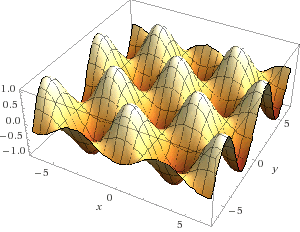
\includegraphics[width=9cm, height=7cm]{images/Terrain/1.png}
              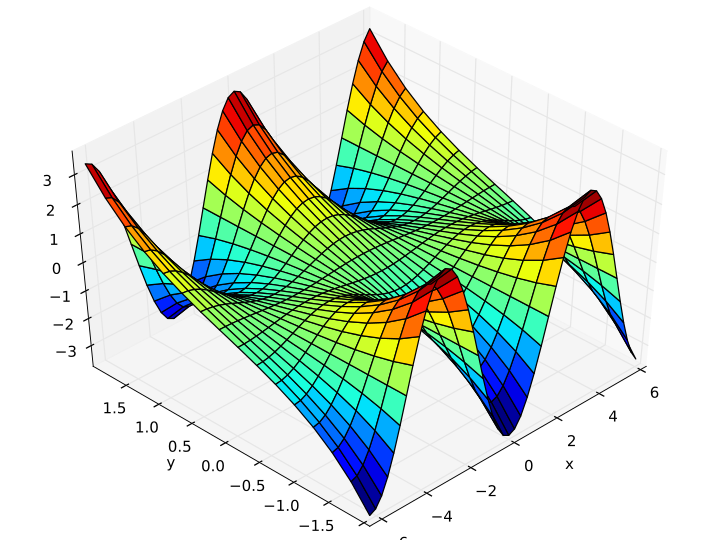
\includegraphics[width=9cm, height=7cm]{images/Terrain/2.png}
              \begin{center}\it The sin(x) * cos(y) and the sinus 3d function\end{center}
            \end{figure}


            \begin{figure}[h]
              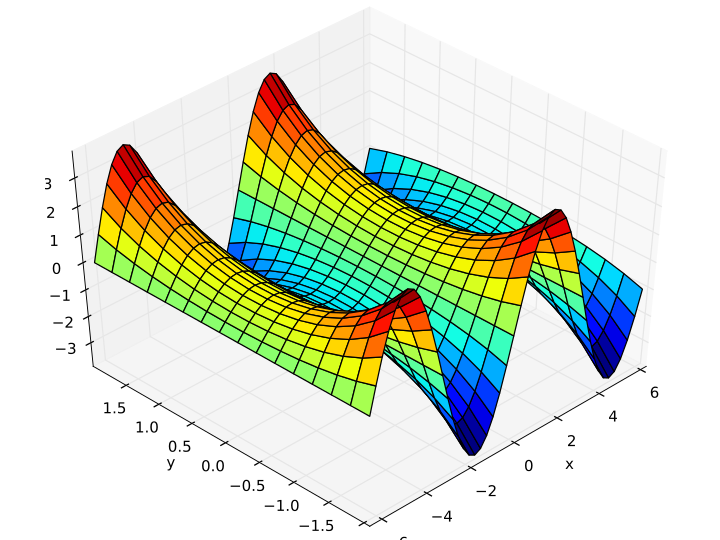
\includegraphics[width=9cm, height=7cm]{images/Terrain/3.png}
              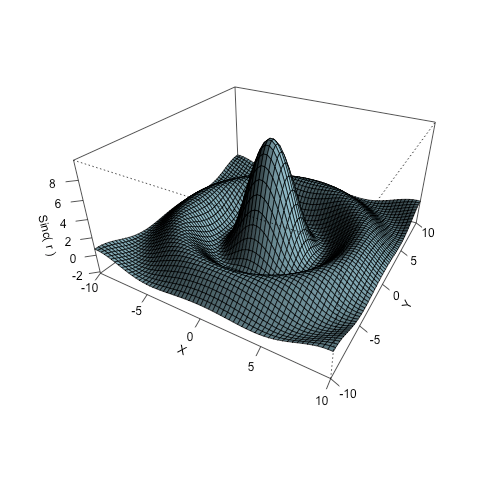
\includegraphics[width=9cm, height=7cm]{images/Terrain/4.png}
              \begin{center}\it The sin(x) function represented in 2d and the sinc 3d function\end{center}
            \end{figure}

            However we quickly understood that using basic functions was not enough. We also wanted random terrain generation however, those functions didn't provide any random factor.\\
            Therefore after some research we ended up using a Perlinh Noise algorithm.
 
      \section{Then Perlin Noise}
        If you look at many things in nature, you will notice that they are fractal. They have various levels of detail. A common example is the outline of a mountain range. It contains large variations in height (the mountains), medium variations (hills), small variations (boulders), tiny variations (stones) . . . you could go on.\\
        Look at almost anything: the distribution of patchy grass on a field, waves in the sea, the movements of an ant, the movement of branches of a tree, patterns in marble, winds. All these phenomena exhibit the same pattern of large and small variations. The Perlin Noise function recreates this by simply adding up noisy functions at a range of different scales.\\

        \subsection{Noise}
          Perlin noise generates coherent noise over a space. Coherent noise means that for any two points in the space, the value of the noise function changes smoothly as you move from one point to the other -- that is, there are no discontinuities.\\

          \begin{figure}[h]
              
\includegraphics[width=9cm, height=7cm]{images/Noise/noncoherent.png}
              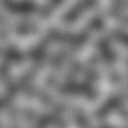
\includegraphics[width=9cm, height=7cm]{images/Noise/coherent.png}
            \end{figure}

          \subsection{Generating Perlin Noise}
            The outline of our algorithm to create noise is very simple. Given an input point P, look at each of the surrounding grid points. In three dimensions there will be eight.\\
            For each surrounding grid point Q, we choose a pseudo-random gradient vector G. It is very important that for any particular grid point you always choose the same gradient vector. 

            Compute the inner product G . (P-Q). This will give the value at P of the linear function with gradient G which is zero at the grid point Q.\\

            When we have 8 of these values. We interpolate between them down to the point, using an S-shaped cross-fade curve (eg: 3t2-2t3) to weight the interpolant in each dimension (we could use a sin function but it would be too slow). This step requires computing 8 S curves, followed by 8-1 linear interpolations (the value has a dimension of degree 1).\\

            We then create an array of the width, height and length of the terrain and fill it with the perlin noise value. We then iterate through the array's 3 dimensions and calculate a noise value for each cells of the array.\\
            The noise value is based on experimentations and advice given by experienced people. At the begining, the value was computed using a simple linear function, however it is now computed using a polynomal function ad two noise arrays :

            \begin{lstlisting}
              
  double noiseValue = (noise[xx, yy, zz]) * noise2[xx, 255 - yy, zz] + noise[xx, yy, zz] - System.Math.Abs(1 / smoothHeight * (yy - smoothHeight - minElevation + 20))

            \end{lstlisting}

            Where smoothHeight correspond to (maxElevation - minElevation) / 2. The noise value computed is a value between -1 and 1 and if it is lower than 0 we consider that it is air.
      \section{Different Islands}
        The smoothHeight value allows us to make different type of Islands, such as plains or even mountains. Because when smoothHeight's value is High, the values computed by noiseValue are higher and tend to be more scattered whereas low values tend to be more concentrated on one level.

        %TODO : image needed
      \section{Decorating the Islands}
        By default, the terrain is just a big cube of stone. However, when generating it, we add air blocks and, solid blocks under air blocks are usually grass (it can be set to another block).\\
        Since we do not want to iterate through the terrain multiple times, this is done when generating the terrain thanks to little algorithm trick :\\

          \begin{lstlisting}  
            for (int xx = 0; xx < this.mIslandSize.x; xx++) {
                for (int zz = 0; zz < this.mIslandSize.z; zz++) {
                  for (int yy = Cst.MAXHEIGHT; yy > 0; yy--) {
          \end{lstlisting}

            We create the terrain from the top, which allow us to check for each block if it's under an air block and if that's true, place a block of grass.\\
            In case the block we just created is solid, we calculate it's distance from the surface and if we told the program beforeHand that there was a special block at the block's particular depth then the type of block will be the one we set, else it's stone.\\
            %TODO : image needed
            Thus in most of the Islands, the first layer is grass and the next two are dirt. The height and the layers are set in a class called Biome.\\

          Once we finished generating the terrain, the next step is to populate it. Which means to add trees or cactus in the different biomes.\\
          Basically we choose a random x and a random z and look for the highest solid block. We then add the cactus and trees.  
      \section{Structures}
          The different structures are usually specific to the biomes and are generated procedurally. As for the cactus and the trees, we get a random point and add the structure.
          We have multiple structures :
          \subsection{Pyramid}
          \subsection{Caverns}
          \subsection{DarkTower}
        \subsubsection{Introduction to the dark tower}
          The dark tower is the biggest structure we made, it is composed of four main towers floating in the sky and is part of the plain biome. This structure is huge because it size can reach 362 blocks on the y axis and has almost 41 floors

        \subsubsection{The main buildings}
          The tower consists in four main buildings whose height vary between 60 and 88 blocks it has about seven floors which can be climbed using the arcane levitator which as it names implies allows you to levitate. Basically if you are on the levitator, it will lift you up to the next floor.

          \begin{center}
            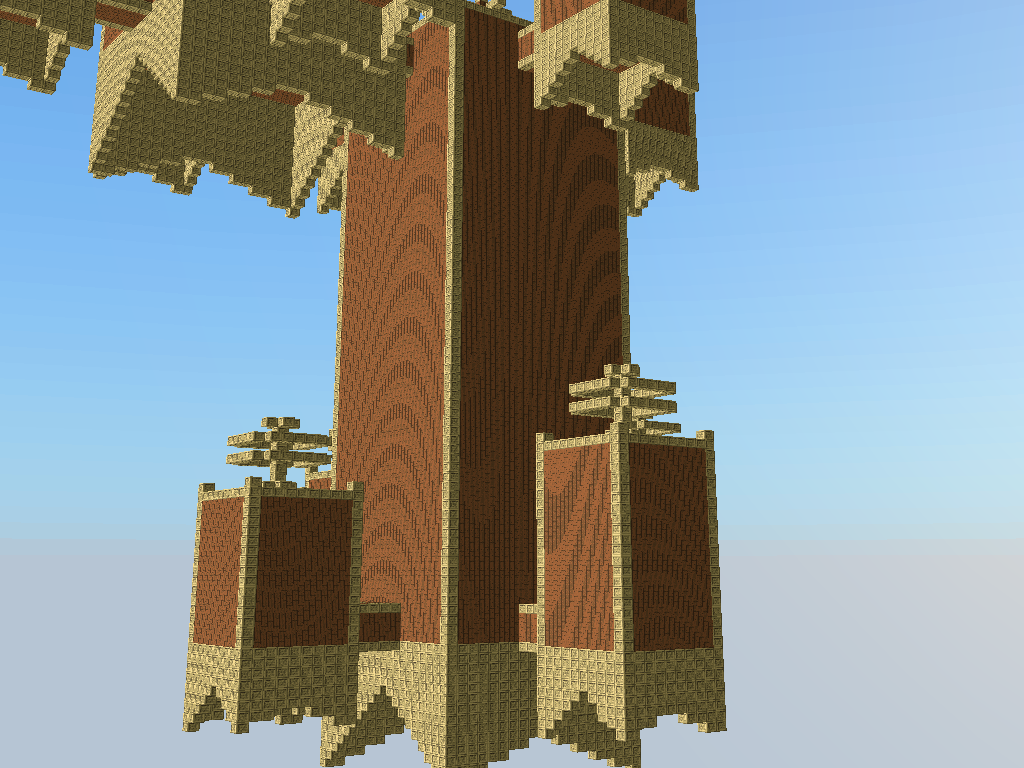
\includegraphics[width=7.5cm]{images/DT/Main.png}
            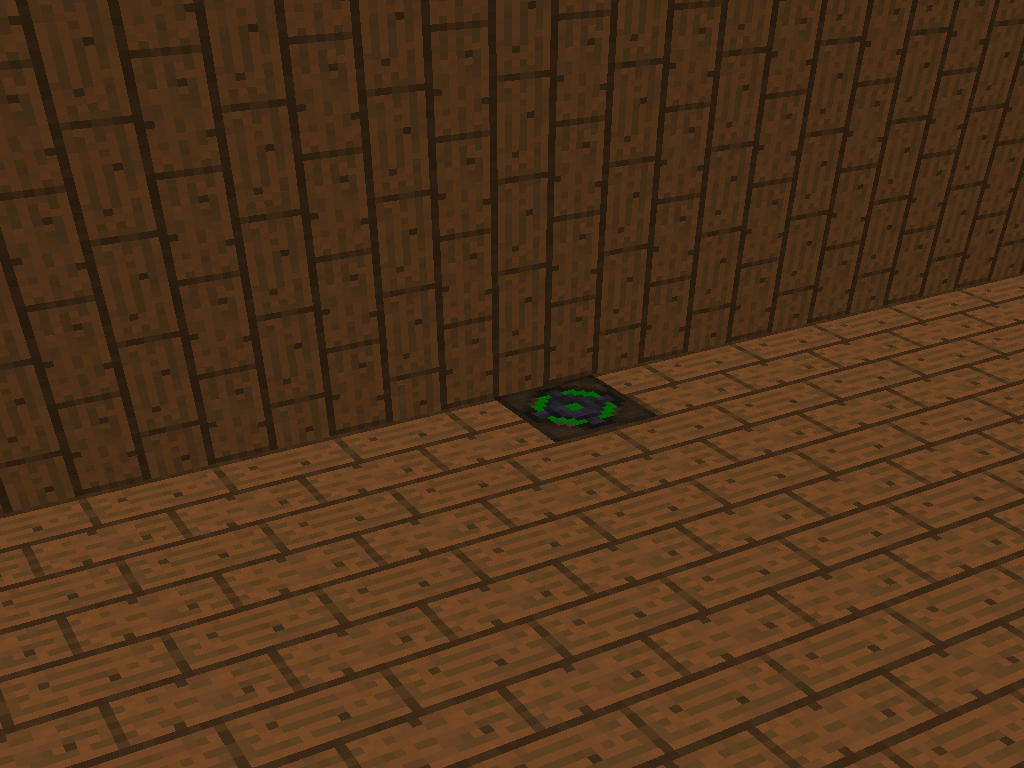
\includegraphics[width=7.5cm]{images/DT/floor.png}
          \end{center}
        finally on the first and last floor of the main tower, bridges connect the main towers to medium towers or another main tower.

        \subsubsection{Bridges}
          Bridges are generated only by the main towers and allows the player to continue climbing the dark tower. One difficulty we encountered while ``building'' the tower was the orientation. Indeed, the algorith to build a bridge facing north is not the same as the algorithm to build a bridge facing west. We struggled to find a way to ``unify'' those algorithm but we finally choose the simplest solution using a switch. Here is the result :
          \begin{center}
            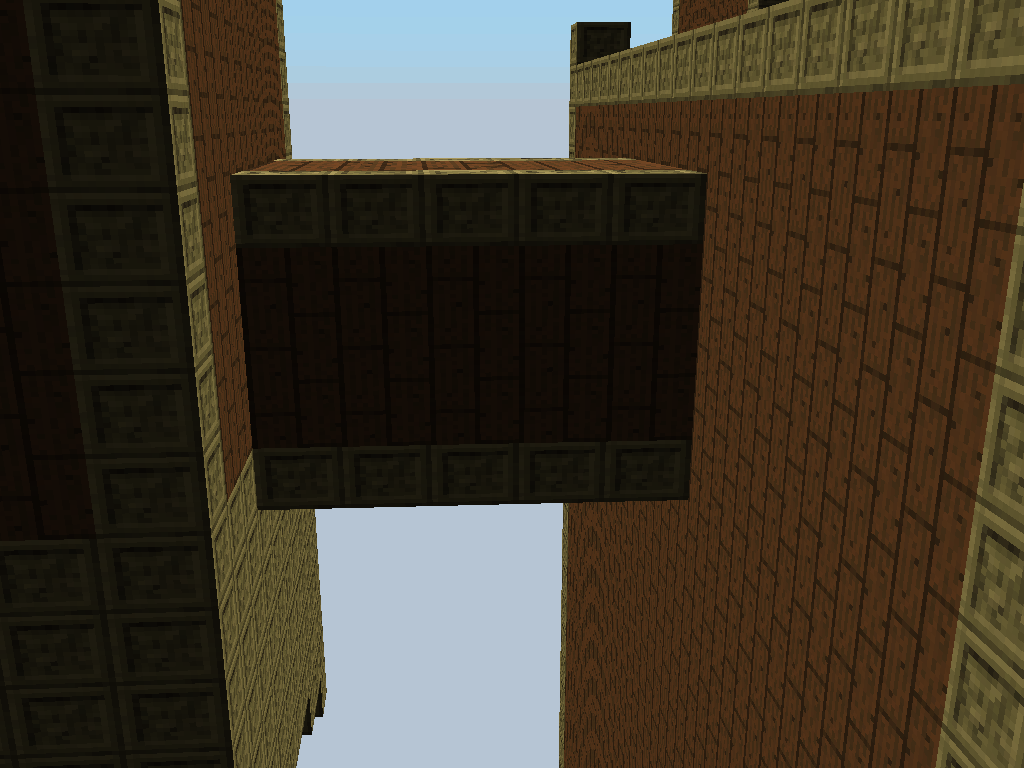
\includegraphics[width=7.5cm]{images/DT/bridge1.png}
            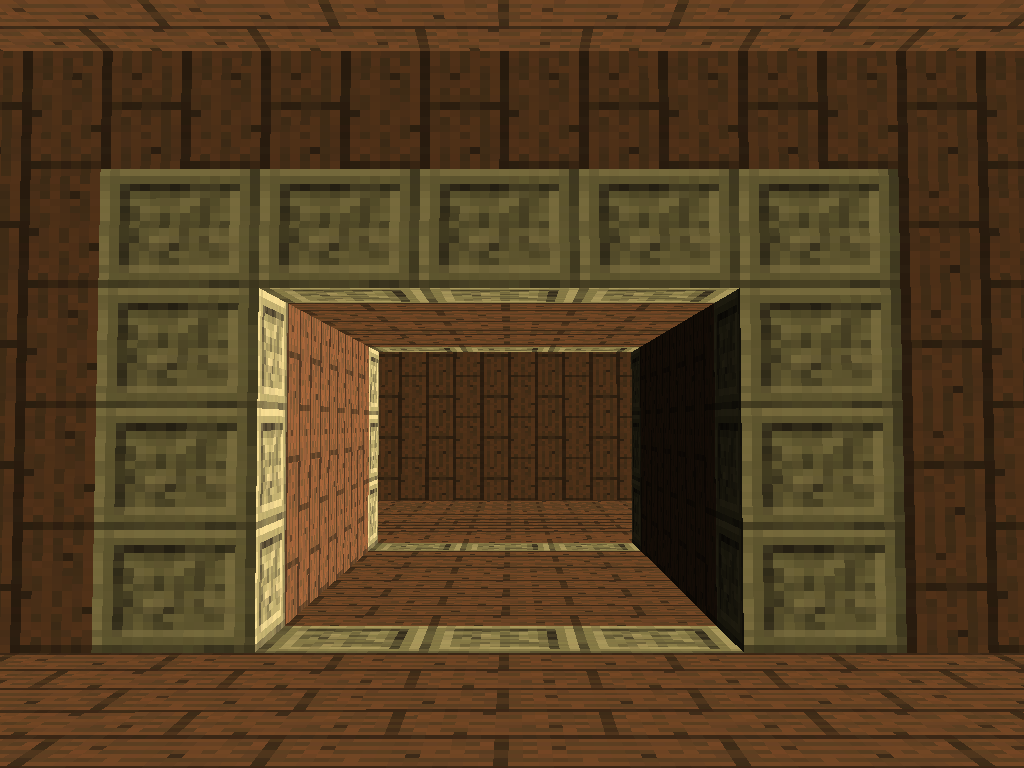
\includegraphics[width=7.5cm]{images/DT/bridge2.png}
          \end{center}

        \subsubsection{Lower towers}
          As I've already said before the main tower are linked by bridges to lower towers their height vary between 15 and 30 blocks and in most of them, the player will find prisonners unit guarded by ennemies and when they are defeated (the ennemies), the prisonners joins the player which can then command them.
          \begin{center}
            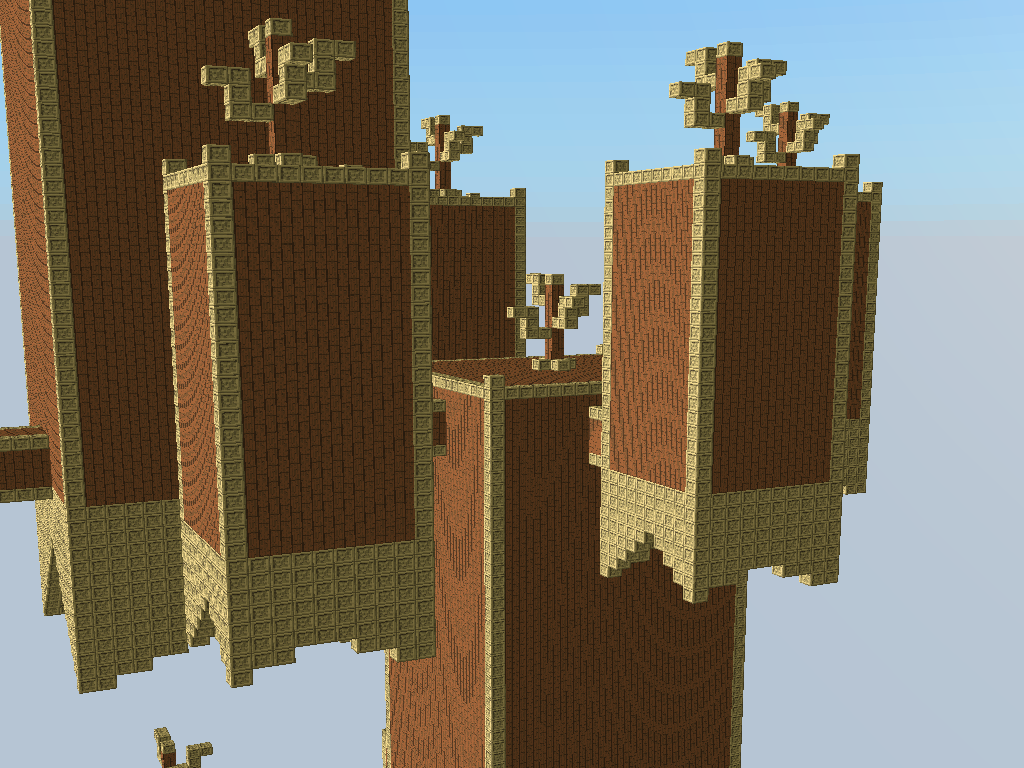
\includegraphics[width=7.5cm]{images/DT/mediumTowers.png}
            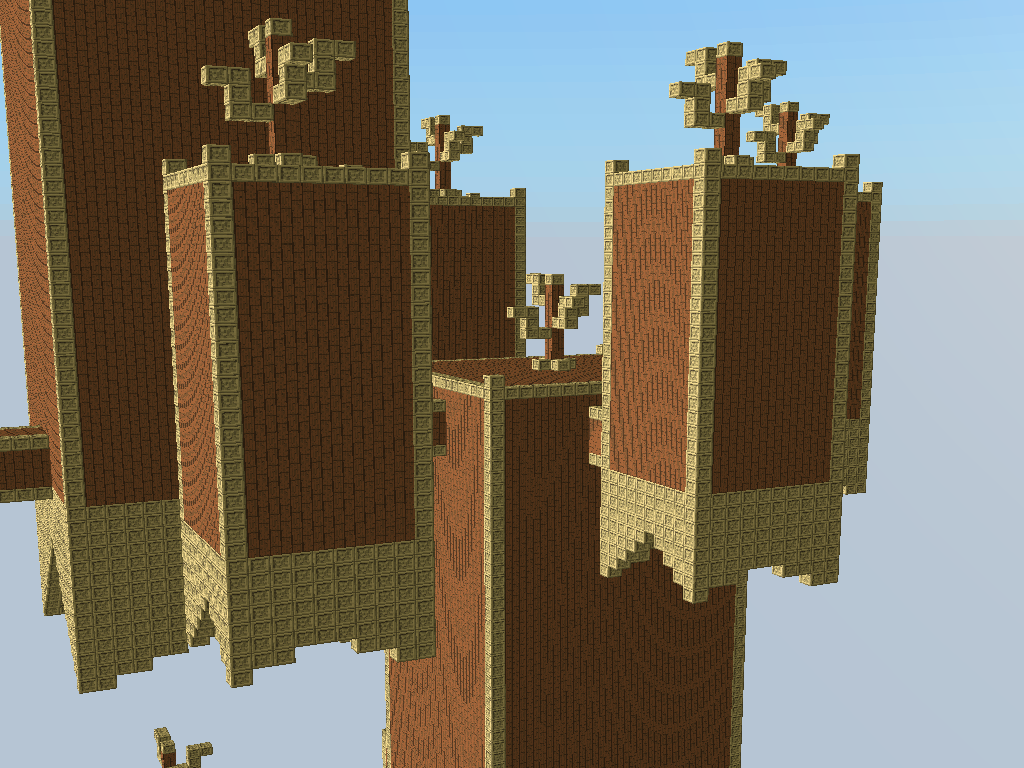
\includegraphics[width=7.5cm]{images/DT/mediumTowers.png} %TODO : Robots
          \end{center}

        \subsubsection{Roofs}
          Among the multiple things which make the tower, one of the most beautiful thing are the structures on the roof, we made 3 of them :
          \begin{center}
            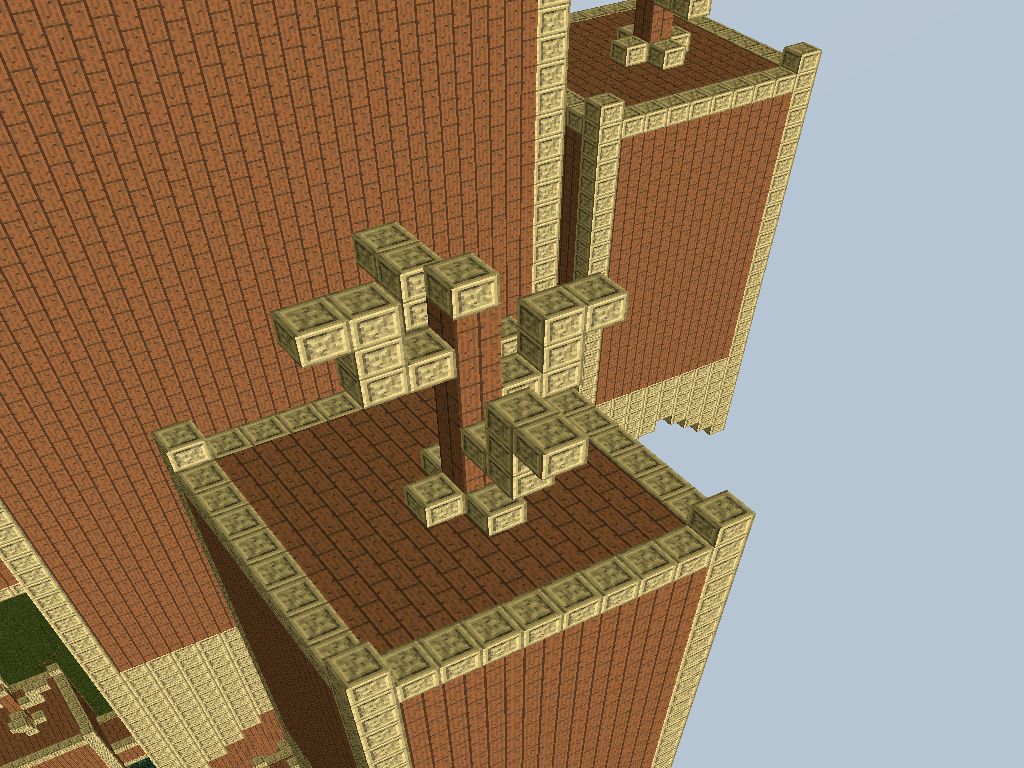
\includegraphics[width=5cm]{images/DT/roof1.png}
            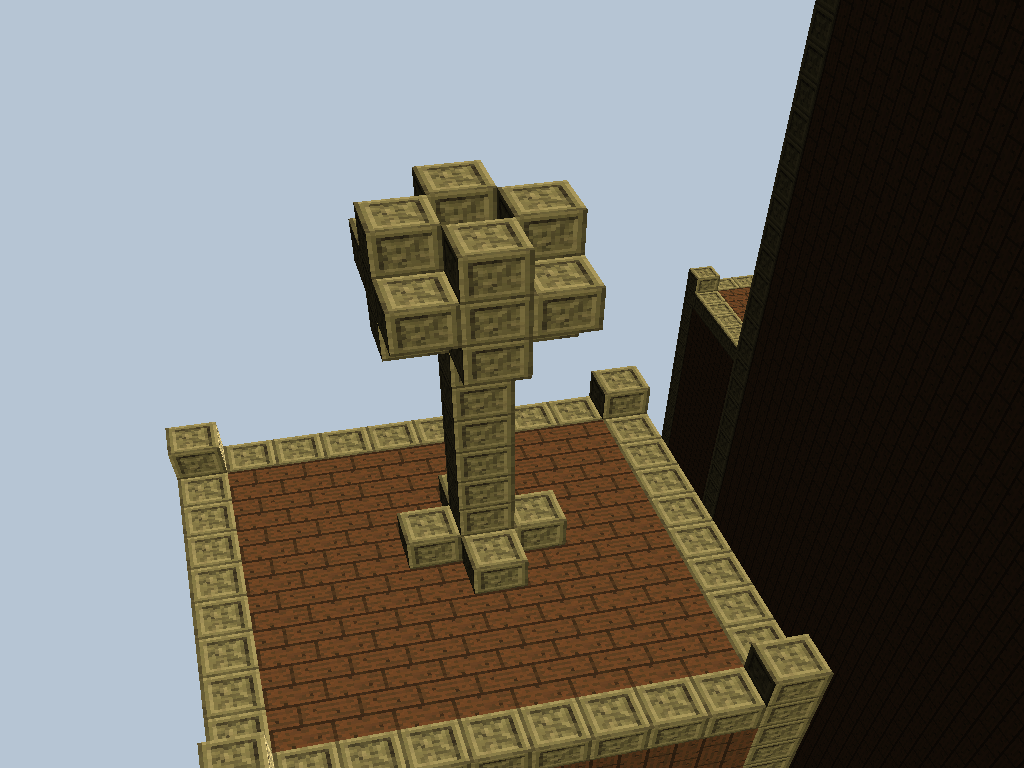
\includegraphics[width=5cm]{images/DT/roof2.png}
            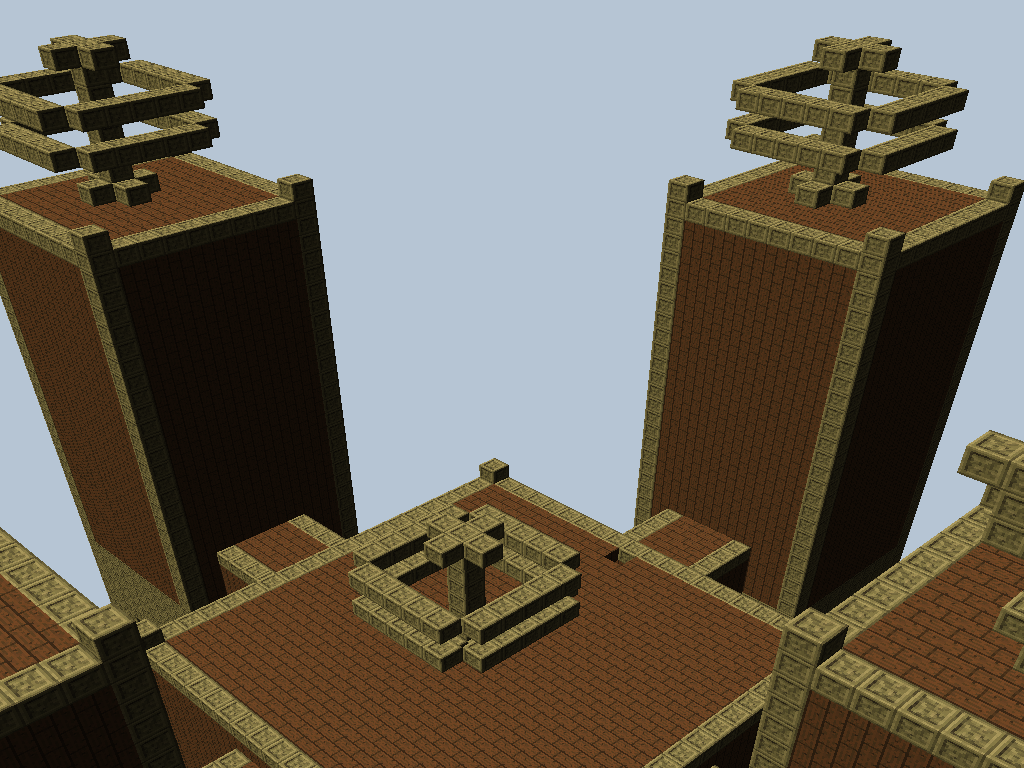
\includegraphics[width=5cm]{images/DT/roof3.png}
          \end{center}
        \subsubsection{DarkBeard}
          Finally, we had to deal with the bottom of the towers. At the beginning we thought that it would stay flat but, we managed to find a function that made the bottom look amazing. We called it the dark beard.

          \begin{center}
            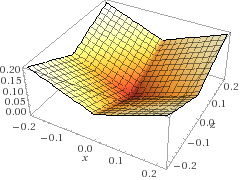
\includegraphics[width=7.5cm]{images/Abs.png}
            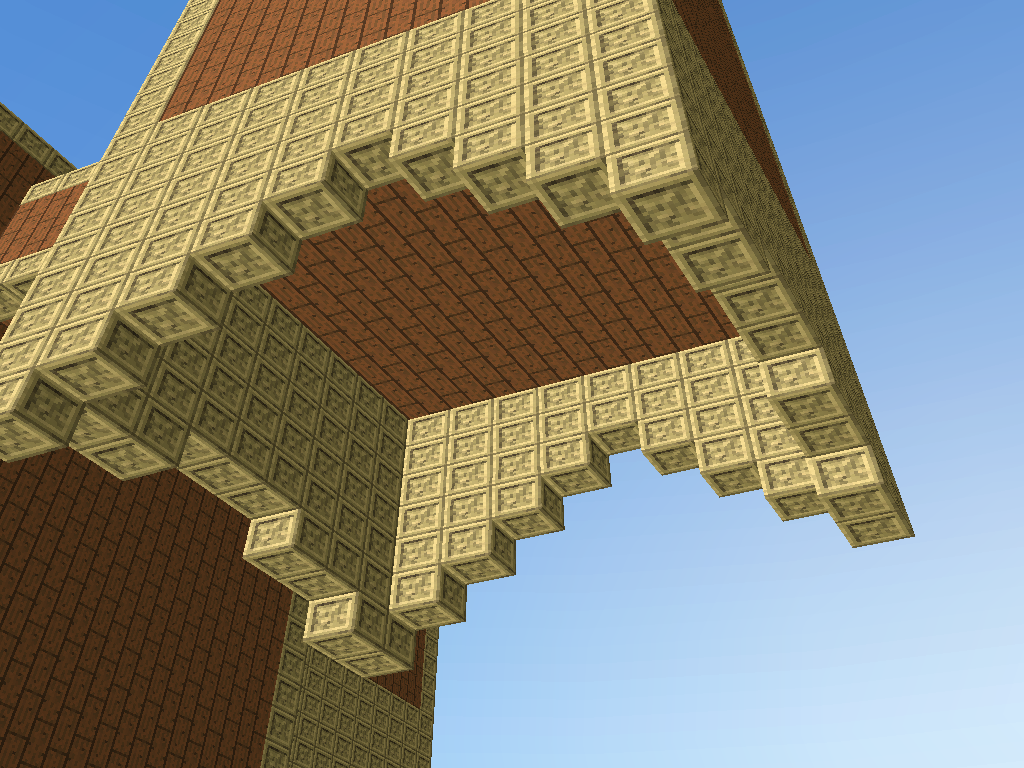
\includegraphics[width=7.5cm]{images/DT/DarkBeard.png} %TODO : Robots
          \end{center}
      \section{Displaying}
        \subsection{Displaying Cubes}
          At first, we thought of dissplaying cubes which where imported entities from blender. \\
          Of course we only displayed visible cubes (cubes which had other cubes adjacent to all his sides were not visibles). However the result was a mere 1 to 10 Frames Per Seconds with a 40 by 40 blocks terrain. In other words a ridiculous amount of Frames Per Seconds.\\

          This lag was mostly caused by the fact that when displaying an entity on the terrain, all it's faces are visible even the ones which you can not see.
        \subsection{Displaying Only Faces}
          Because of the lag caused by this method, we had no other choice but to find another way of displaying the terrain.\\
          Thus we came up with the following idea :\\
          We created in the code the six different faces which are composing a block.\\
          Thanks to Ogre, this was a fairly easy process, creating an object whith little triangle composing it in the code is no more than seven line!
          \begin{lstlisting}

ManualObject block = new ManualObject("name");
block.Begin("texture here", RenderOperation.OperationTypes.OT_TRIANGLE_LIST);
    block.Position(new Vector3(0,   0,     0));
    block.Position(new Vector3(0,   100,   0));
    block.Position(new Vector3(100, 0,     0));
    block.Position(new Vector3(100, 100,   0));

    block.Triangle(0, 1, 2);
    block.Triangle(1, 2, 3);
block.End();
        \end{lstlisting}

        Of course there are other things we have to do such as specifying the coordinates of the textures or the normals (normals are used in order to cast shadow on the surface).\\
 
        Once the six different faces were created, we would iterate through the terrain and each time we would find a visible face (face that is not hidden by another block), we would make a copy of the created face, assign it a texture and then, place it at the correct position.

        \begin{center}
            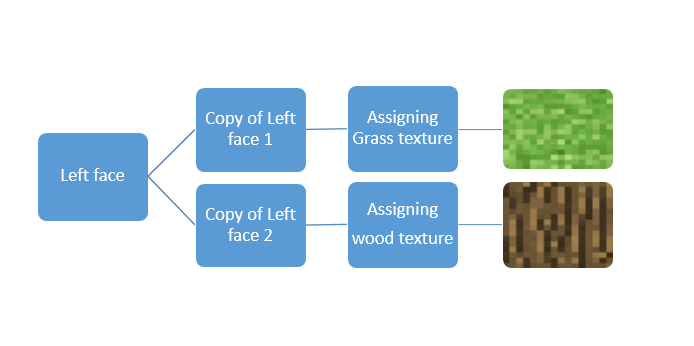
\includegraphics[width=16cm]{images/Display.png}
        \end{center}

        With this system, we ended up having better Frames Per Seconds than the previous displaying system, but this count was very variable and depended on how many entities were displayed on the sreen.\\
        
        Basically the the terrain we could display was bigger, but we needed to stop displaying entities at a certain distance (usually 3000 pixels) and our terrain couldn't bigger than 12 chunks of 16 blocks.\\

        Frames Per Seconds were usually between 15 and 30, and as you might expect, we were a bit disapointed because under 24 Frames Per Seconds, animations are uneven or worse ``choppy'' movement or animations, and the frame rate was more often under 25 than above.\\

        \subsection{A better display system}
          Though we had a ``working'' display system we wanted it to be better, we also wanted higher Frames Per Seconds. Actually the moment we made the second we were already thinking of a new algorithm.\\

          The basic gist of it is as follows : we create a ManualObject (as defined higher) in which we don't add any point for each different textures.\\
          We then iterate through terrain looking for visisble faces. When we find one, we add, the face to the manual object corresponding to it's texture.\\
          Once we finished iterating through the terrain, we close each manual object (by calling the End() method) and then display them.\\

          Basically, each visible faces with the same texture of the terrain are part of the same material. Thus, instead of thousands of entities (1 per visible face) we only have about 20 entities displayed at all times on the screen.\\

          The end result is, terrain of about 121 chunks for plains Biomes and maximum 2000 (mostly for the mountain biome) with an average frame rate of 60 on Epita's computers!\\

          This system is of course more complicated than explained and has consequences on other parts (especially adding and removing blocks), but it was totally worth the cost, we increased the maximum  frame rate by 30 (sometimes more). Also, the Islands size were trippled, getting from 4*4 to 12*12 (on the x and z coordinates) and can even be increased to 30 * 30.\\
          This means that if we assimilated the terrain as one continuous layer of block (with a height of 1) we would have : 30 * 30 * 16 * 16 = 230400 cubes, counting only top faces and bottom faces : 460800 faces and 921600 triangles, thus around 1 000 000 triangles (with about 60 FPS since the height is only 1).\\
          And we beleive we could display even more cubes!\\

      \section{Save and Load}
        Saving and loading the terrain would've been too easy if we had choosen to write it in a text file!\\
        Basically we iterate through the terrain with 3 for (x, y, z) from 0 to the max size and we only need to write the id of the block, which is a byte.\\
        The only thing we need to do is at the begining of the file write the max-size in x, thhe max-size in the and the max-size in y. Once this is done, we iterate through the terrain using a FileStream and it's methode WriteByte.\\

        As for the reading part, obviously we begin by reading the max-size values in x, y, z and once this is done, we iterate through the file using ReadByte and build the terrain according to the input we read. Nothing really technical!\\
      
       The results talk for themselves, for 100 000 blocks = 100 000 bytes = 100 ko. which would be around the number of blocks contained in a 15 * 15 island. So tiny files for big Islands!\\

    \chapter{\textcolor{blue}{Physics}}
      \section{Collisions} %Romain à toi de faire plusieurs parties
      \section{Fall}
    \chapter{\textcolor{blue}{Gameplay}}
      \section{Exploring the terrain}
      \section{Adding Blocks}
      \section{Removing Blocks}
      \section{Inventory, Selector}
      \section{Crafting}
    \chapter{\textcolor{blue}{Strategy}}
      \section{Build your own Base}
      \section{Buy your army of Robots}
      \section{Fight against foes}
      \section{PathFinding}
    \chapter{\textcolor{blue}{Graphics}}
      \section{High / Low definition}
      \section{Sinbad's skins}
      \section{Particles}
    \chapter{\textcolor{blue}{Scenario Editor}}
      \section{Basic Idea}
      \section{Structures}
      \section{Scripting}
    \chapter{\textcolor{blue}{Sound Engine}}
    \chapter{\textcolor{blue}{Website}}
    \chapter{\textcolor{blue}{Conclusion}}
    
\end{document}